\documentclass{beamer}
%
% Choose how your presentation looks.
%
% For more themes, color themes and font themes, see:
% http://deic.uab.es/~iblanes/beamer_gallery/index_by_theme.html
%
\mode<presentation>
{
  \usetheme{default}      % or try Darmstadt, Madrid, Warsaw, ...
  \usecolortheme{default} % or try albatross, beaver, crane, ...
  \usefonttheme{default}  % or try serif, structurebold, ...
  \setbeamertemplate{navigation symbols}{}
  \setbeamertemplate{caption}[numbered]
} 

\usepackage[english]{babel}
\usepackage[utf8x]{inputenc}

\newcommand{\mdh}{\texttt{multi\-dupe\-hack}}
\newcommand{\etal}{\emph{et al.}}
\newcommand{\aeth}{\texttt{Aetheris}}
\newcommand{\domp}{\texttt{DP}}
\newcommand{\cpsky}{\texttt{CP+SKY}}



%%%%%%%%%%%%%%%%%%%%%%%%%%%%%%%%%%%%%%%%%%%%%%%%%%%%%%%%%%%%%%%%%%%%%%%%%%%%%%%%

\title[Mining Skypatterns]{Mining Skypatterns in Uncertain Tensors}
\subtitle{dupe hacks in the sky}
\author{Nicolas Nadisic}
\institute{INSA Lyon\\ Universidade Federal de Minas Gerais}
\date{June 29$^{\text{th}}$ 2018}

\begin{document}

\begin{frame}
  \titlepage
\end{frame}

% Uncomment these lines for an automatically generated outline.
\begin{frame}{Outline}
  \tableofcontents
\end{frame}

%%%%%%%%%%%%%%%%%%%%%%%%%%%%%%%%%%%%%%%%%%%%%%%%%%%%%%%%%%%%%%%%%%%%%%%%%%%%%%%%
\section{Uncertain tensors}
\begin{frame}{Outline}
  \tableofcontents[currentsection]
\end{frame}

\begin{frame}{From the 0/1 matrix to the uncertain tensor}
\begin{figure}[htp]
\centering
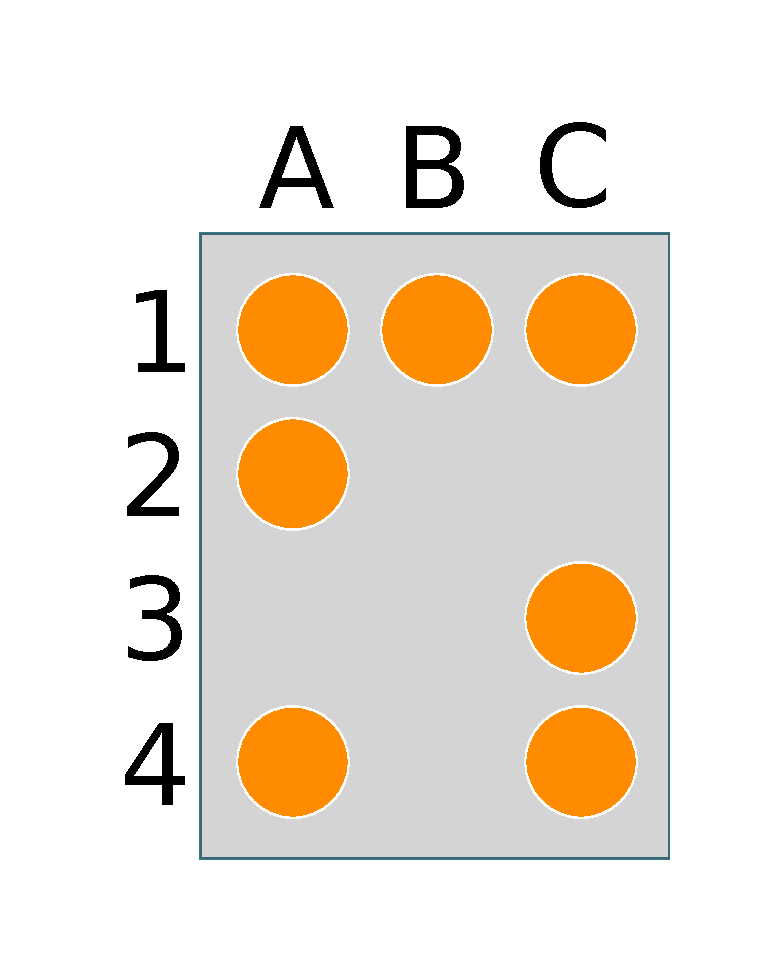
\includegraphics[width=.3\textwidth]{bin-matrix.pdf}\hfill
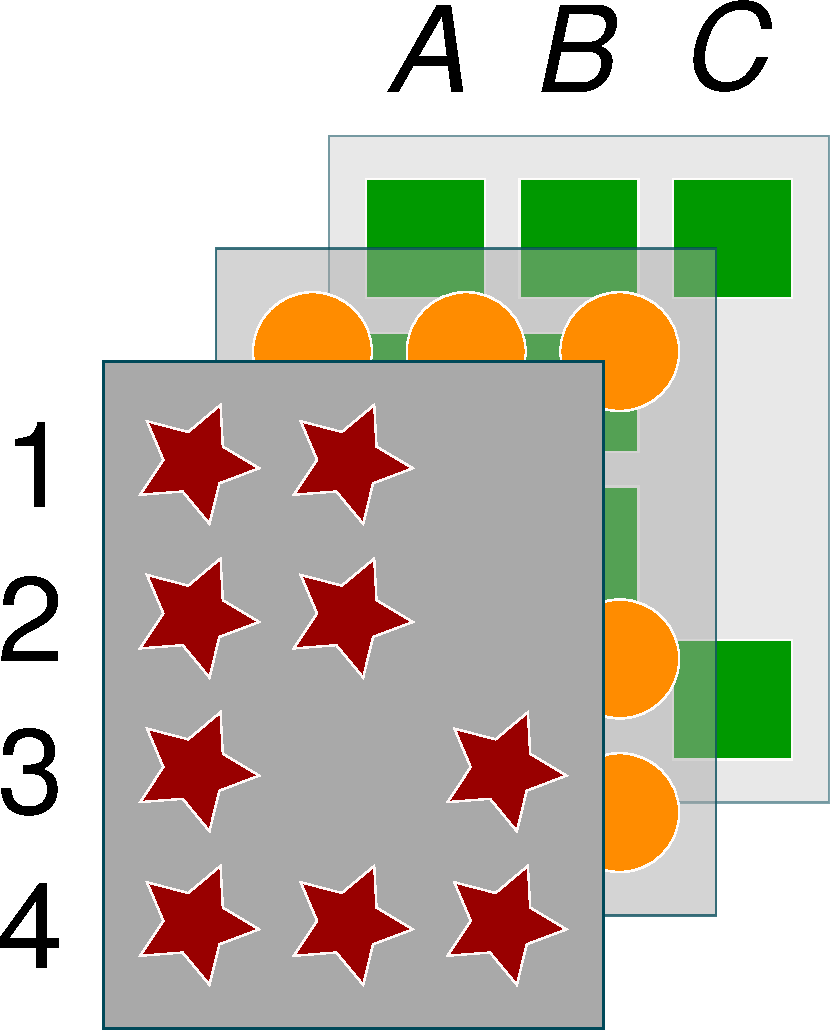
\includegraphics[width=.3\textwidth]{cube.pdf}\hfill
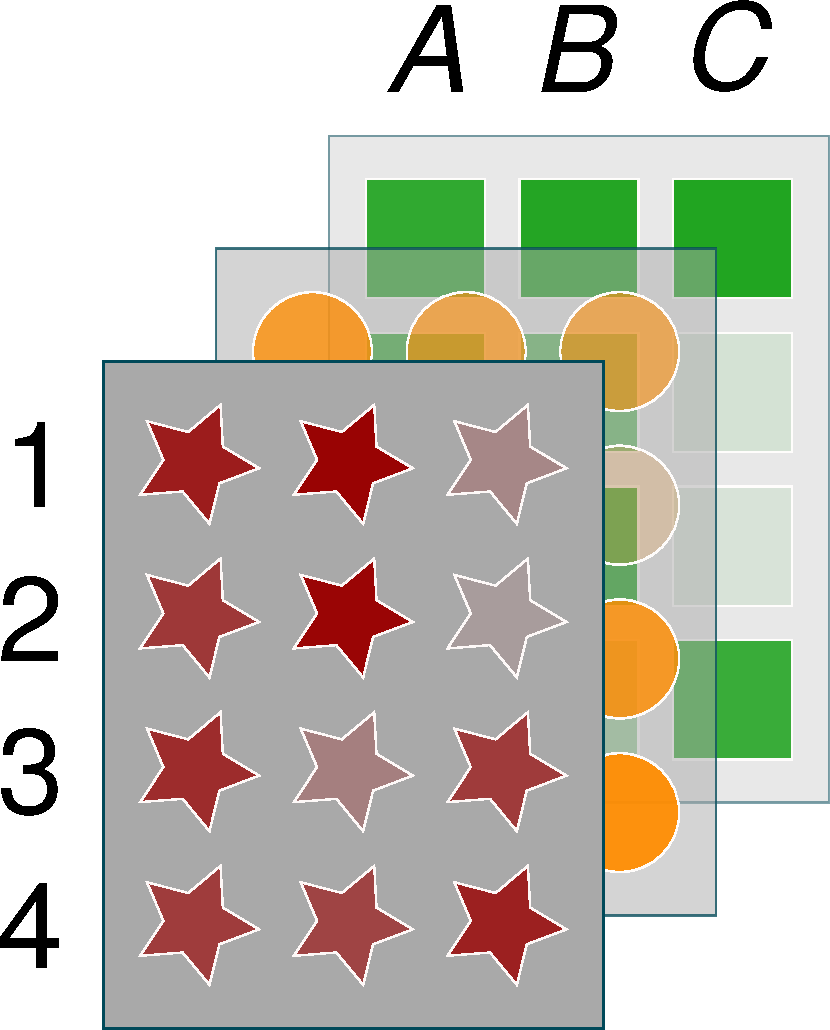
\includegraphics[width=.3\textwidth]{probabilistic_cube.pdf}
\caption{0/1 matrix --- 0/1 tensor --- uncertain tensor}
\end{figure}
\end{frame}

%%%%%%%%%%%%%%%%%%%%%%%%%%%%%%%%%%%%%%%%%%%%%%%%%%%%%%%%%%%%%%%%%%%%%%%%%%%%%%%%
\section{Skyline and skypatterns: a state of the art}
\begin{frame}{Outline}
  \tableofcontents[currentsection]
\end{frame}
% Histoire depuis Pareto, Borzony, Soulet, Ugarte
% Notre contribution

\begin{frame}{Sky is the limit}
  \framesubtitle{Pareto domination}
  \begin{figure}[htp]
    \centering
    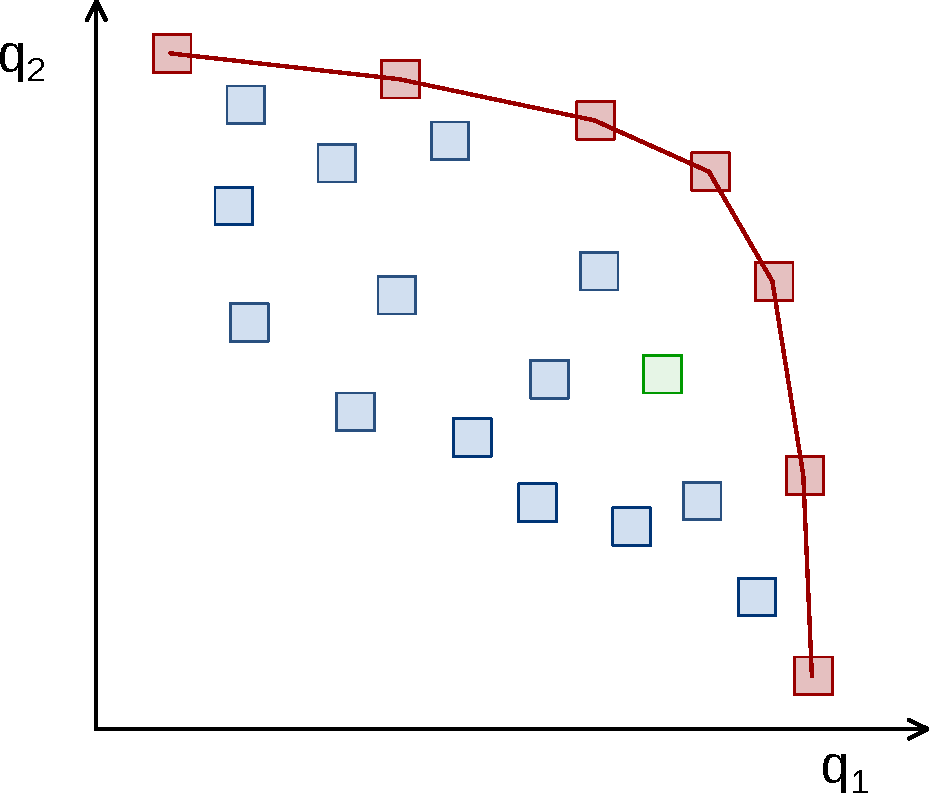
\includegraphics[width=0.6\textwidth]{domination.pdf}
    \caption{A Pareto optimal front of elements w.r.t.\ two measures.}
  \end{figure}  
\end{frame}

\begin{frame}{Sky is the limit}
  \framesubtitle{Pareto domination}
  \begin{definition}[Pareto domination]
  \label{def:pareto}
  An element $X$ \emph{dominates} an element
  $Y$ with respect to a set of measures
  $M$, denoted $X \succ_M Y$, if and only if $$\forall m \in M, m(X)
  \geq m(Y) \wedge \exists m \in M, m(X) > m(Y)$$.
 \end{definition}
 \pause
 \begin{definition}[Pareto optimality]
  Given a set of elements $T$, and a set of
  measures $M$, an element $X \in T$ is Pareto-optimal if and only if it is \emph{non dominated}, i.e.\
    $$\forall Y \in T, Y \nsucc_M X $$
  \end{definition}

The group of all Pareto-optimal elements is called \emph{Pareto optimal front} or \emph{Pareto set}

\end{frame}

\begin{frame}{Sky is the limit}
  \framesubtitle{The skyline operator}
  \begin{itemize}
  \item "The skyline operator", Börzsöny \etal{}, 2001
  \item SQL query
  \item Return tuples that are Pareto optimal w.r.t.\ a set of attributes
  \end{itemize}
\end{frame}

\begin{frame}{Sky is the limit}
  \framesubtitle{The skyline operator}
  \begin{figure}[htp]
  \centering
  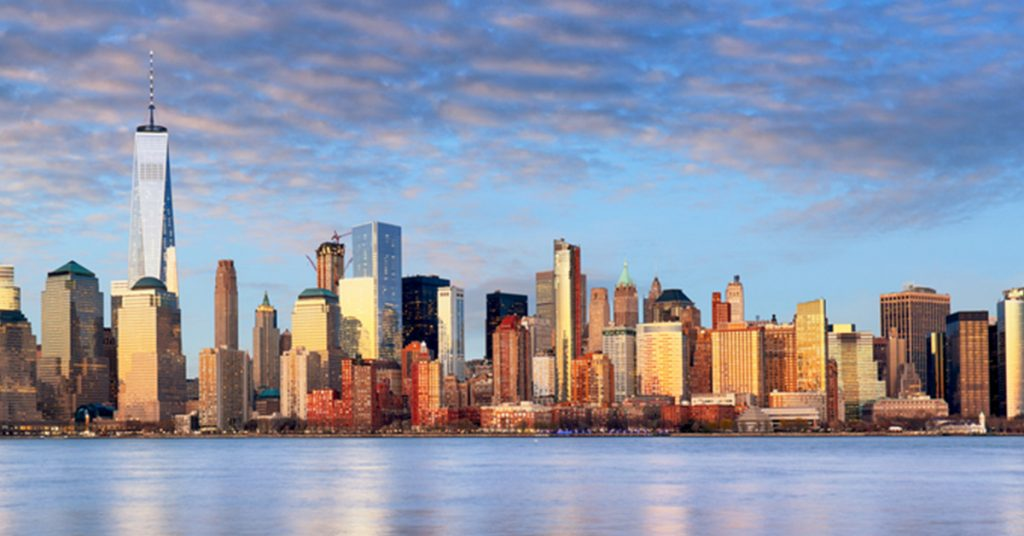
\includegraphics[width=\textwidth]{manhattan.jpg}
  \caption{The skyline of Manhattan}
  \end{figure} 
\end{frame}

\begin{frame}{Sky is the limit}
  \framesubtitle{Skyline patterns → skypatterns}
  \begin{itemize}
  \item "Mining dominant patterns in the sky", Soulet \etal{}, 2011
  \item \aeth{} algorithm
  \item Generalization of the skyline query to itemset mining
  \pause
  \item Optimize simultaneously various measures on the patterns
  \item No need for user-defined thresholds
  \pause
  \item Post-process approach → lack of performance
  \end{itemize}
\end{frame}

%%%%%%%%%%%%%%%%%%%%%%%%%%%%%%%%%%%%%%%%%%%%%%%%%%%%%%%%%%%%%%%%%%%%%%%%%%%%%%%%
\section{Preliminary definitions}
\begin{frame}{Outline}
  \tableofcontents[currentsection]
\end{frame}

\begin{frame}[allowframebreaks]{Definitions}
  \begin{definition}[ET-$n$-set]
  Given an uncertain tensor $T$ and $n$ noise-tolerance thresholds
  $(\epsilon_1, \dots, \epsilon_n) \in \mathbb{R}_+^n$, a pattern
  $(X_1, \dots, X_n)$ is an ET-$n$-set in $T$ if and only if $\forall i
  \in \{1, \dots, n\}$, $\forall x \in X_i$, $\sum_{t \in \prod_{i =
      1}^n X_i\text{ s.t. }t_i = x} 1 - T_t \leq \epsilon_i$, where
  $t_i$ denotes the $i^{\text{th}}$ component of the $n$-tuple $t$.
  \end{definition}
  
  \begin{definition}[Measure]
  \label{def:measure}
  A \emph{measure} is a function of whose domain is $\prod_{i = 1}^n
  2^{D_i}$ and whose codomain is $\mathbb{R}$.
  \end{definition}

\framebreak  
  \begin{definition}[External-data-access function]
  Given $I \subseteq \{1, \dots, n\}$, an \emph{external-data-access
    function over $I$} is a function whose domain is $\prod_{i \in I}
  D_i$ and whose codomain is $\mathbb{R}$.
  \end{definition}

  \begin{block}{Ex: the utility measure}
  Given $I \subseteq \{1, \dots, n\}$ and an external-data-access
  function $u$ over $I$, the \emph{utility} is the measure $(X_1,
  \dots, X_n) \mapsto \sum_{t \in \prod_{i \in I} X_i} u(t)$.
  \end{block}
  
\framebreak
  \begin{definition}[Rewriting]
  $m'$ is a \emph{rewriting} of a measure $m$ if and only if it is a
  function, whose domain is $\left(\prod_{i = 1}^n 2^{D_i}\right)^2$,
  whose codomain is $\mathbb{R}$, and that is such that $\forall X \in
  \prod_{i = 1}^n 2^{D_i}$, $m'(X, X) = m(X)$.
  \end{definition}
  
   \begin{block}{Ex: rewriting the utility measure}
  Here is, for example, a rewriting $m'_{\text{utility}}$ of the utility
measure $m_{\text{utility}}$:
  \begin{equation*}
  (X^a_1, \dots, X^a_n, X^m_1, \dots, X^m_n) \mapsto \sum_{\substack{t
      \in \prod_{i \in I} X_i^a\\\text{such that }u(t) < 0}} u(t) +
  \sum_{\substack{t \in \prod_{i \in I}X_i^m\\\text{such that }u(t) >
      0}} u(t) \enspace .
  \end{equation*}
  \end{block}
  
\framebreak
  \begin{definition}[Piecewise (anti-)monotonicity]
  A measure $m$ is piecewise (anti-)monotone if and only if there exists
  a rewriting $m'$ of $m$ such that:\\
  $\forall U \in \prod_{i = 1}^n 2^{D_i}$, $\forall X \in \prod_{i =
  1}^n 2^{U_i}$, $\forall L \in \prod_{i = 1}^n 2^{X_i}$, $m(X) \leq
  m'(L, U)$.
  \end{definition}


  
\end{frame}


%%%%%%%%%%%%%%%%%%%%%%%%%%%%%%%%%%%%%%%%%%%%%%%%%%%%%%%%%%%%%%%%%%%%%%%%%%%%%%%%
\section{The \mdh{} algorithm}
\begin{frame}{Outline}
  \tableofcontents[currentsection]
\end{frame}

\begin{frame}{\mdh{} is not a dupehack}
  % Présentation multidupehack : pam, arbre, pseudo code 
  
\end{frame}

%%%%%%%%%%%%%%%%%%%%%%%%%%%%%%%%%%%%%%%%%%%%%%%%%%%%%%%%%%%%%%%%%%%%%%%%%%%%%%%%
\section{Mining skypatterns with \mdh{}}
\begin{frame}{Outline}
  \tableofcontents[currentsection]
\end{frame}

\begin{frame}{Dupe hacks in the sky}
  % Arbre, pseudocode
  % Notre contribution
  
\end{frame}

%%%%%%%%%%%%%%%%%%%%%%%%%%%%%%%%%%%%%%%%%%%%%%%%%%%%%%%%%%%%%%%%%%%%%%%%%%%%%%%%
\section{Experimental study}
\begin{frame}{Outline}
  \tableofcontents[currentsection]
\end{frame}

\subsection{Skypatterns in 0/1 matrices: a comparative study}

\begin{frame}{Comparative study}

\end{frame}


%%%%%%%%%%%%%%%%%%%%%%%%%%%%%%%%%%%%%%%%%%%%%%%%%%%%%%%%%%%%%%%%%%%%%%%%%%%%%%%%
\subsection{Skypatterns in real-life uncertain tensors}

\begin{frame}{Twitch}
  \framesubtitle{Experimental protocol}

\end{frame}

\begin{frame}{Twitch}
  \framesubtitle{Results}

\end{frame}


\begin{frame}{Vélo'v}
  \framesubtitle{Experimental protocol}
  
\end{frame}

\begin{frame}{Vélo'v}
  \framesubtitle{Results}
  
\end{frame}


%%%%%%%%%%%%%%%%%%%%%%%%%%%%%%%%%%%%%%%%%%%%%%%%%%%%%%%%%%%%%%%%%%%%%%%%%%%%%%%%
\section{Conclusion}
\begin{frame}{Outline}
  \tableofcontents[currentsection]
\end{frame}

\begin{frame}{Conclusion}
  Our contributions:
  \begin{itemize}
  \item State of the art
  \item Generalization of the skypattern mining problem
  \item Design of an efficient and versatile algorithm
  \item Implementation by extending \mdh{}
    \begin{itemize}
    \item Faster than the competitors, despite greater generality
    \item Able to mine relevant pattern in real-life situations
    \end{itemize}
  \end{itemize}
\end{frame}

\begin{frame}{}
  \begin{figure}[htp]
    \centering
    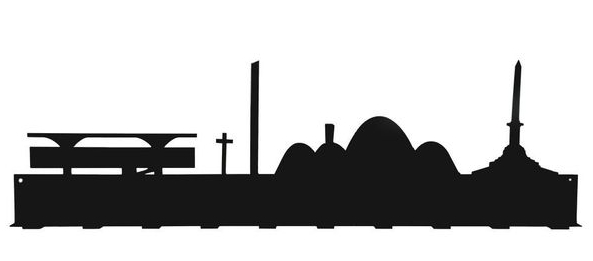
\includegraphics[width=\textwidth]{bh-skyline.jpg}
  \end{figure} 
\end{frame}



%%%%%%%%%%%%%%%%%%%%%%%%%%%%%%%%%%%%%%%%%%%%%%%%%%%%%%%%%%%%%%%%%%%%%%%%%%%%%%%%
\end{document}
%%%%%%%%%%%%%%%%%%%%%%%%%%%%%%%%%%%%%%%%%%%%%%%%%%%%%%%%%%%%%%%%%%%%%%%%%%%%%%%% 
%%%%%%%%%%%%%%%%%%%%%%%%%%%%%%%%%%%%%%%%%%%%%%%%%%%%%%%%%%%%%%%%%%%%%%%%%%%%%%%%
%%%%%%%%%%%%%%%%%%%%%%%%%%%%%%%%%%%%%%%%%%%%%%%%%%%%%%%%%%%%%%%%%%%%%%%%%%%%%%%%

% \section{Some \LaTeX{} Examples}

% \subsection{Tables and Figures}

% \begin{frame}{Tables and Figures}

% \begin{itemize}
% \item Use \texttt{tabular} for basic tables --- see Table~\ref{tab:widgets}, for example.
% \item You can upload a figure (JPEG, PNG or PDF) using the files menu. 
% \item To include it in your document, use the \texttt{includegraphics} command (see the comment below in the source code).
% \end{itemize}

% % Commands to include a figure:
% %\begin{figure}
% %\includegraphics[width=\textwidth]{your-figure's-file-name}
% %\caption{\label{fig:your-figure}Caption goes here.}
% %\end{figure}

% \begin{table}
% \centering
% \begin{tabular}{l|r}
% Item & Quantity \\\hline
% Widgets & 42 \\
% Gadgets & 13
% \end{tabular}
% \caption{\label{tab:widgets}An example table.}
% \end{table}

% \end{frame}

% \subsection{Mathematics}

% \begin{frame}{Readable Mathematics}

% Let $X_1, X_2, \ldots, X_n$ be a sequence of independent and identically distributed random variables with $\text{E}[X_i] = \mu$ and $\text{Var}[X_i] = \sigma^2 < \infty$, and let
% $$S_n = \frac{X_1 + X_2 + \cdots + X_n}{n}
%       = \frac{1}{n}\sum_{i}^{n} X_i$$
% denote their mean. Then as $n$ approaches infinity, the random variables $\sqrt{n}(S_n - \mu)$ converge in distribution to a normal $\mathcal{N}(0, \sigma^2)$.

% \begin{block}{Examples}
% Some examples of commonly used commands and features are included, to help you get started.
% \end{block}

% \end{frame}

% \end{document}
